%%%%%%%%%%%%%%%%%%%%%%%%%%%%%%%%%%%%%%%%%
% Diaz Essay
% LaTeX Template
% Version 2.0 (13/1/19)
%
% This template originates from:
% http://www.LaTeXTemplates.com
%
% Authors:
% Vel (vel@LaTeXTemplates.com)
% Nicolas Diaz (nsdiaz@uc.cl)
%
% License:
% CC BY-NC-SA 3.0 (http://creativecommons.org/licenses/by-nc-sa/3.0/)
%
%%%%%%%%%%%%%%%%%%%%%%%%%%%%%%%%%%%%%%%%%

%----------------------------------------------------------------------------------------
%	PACKAGES AND OTHER DOCUMENT CONFIGURATIONS
%----------------------------------------------------------------------------------------

\documentclass[12pt]{diazessay} % Font size (can be 10pt, 11pt or 12pt)

%----------------------------------------------------------------------------------------
%	TITLE SECTION
%----------------------------------------------------------------------------------------

\title{\textbf{A brief history of machine learning} \\ {\Large\itshape}} % Title and subtitle

\author{\textbf{Douglas Mesquita} \\ \textit{CCT College}} % Author and institution

\date{\today} % Date, use \date{} for no date

%----------------------------------------------------------------------------------------

\begin{document}

\maketitle % Print the title section

%----------------------------------------------------------------------------------------
%	ABSTRACT AND KEYWORDS
%----------------------------------------------------------------------------------------

%\renewcommand{\abstractname}{Summary} % Uncomment to change the name of the abstract to something else

\begin{abstract}
Morbi tempor congue porta. Proin semper, leo vitae faucibus dictum, metus mauris lacinia lorem, ac congue leo felis eu turpis. Sed nec nunc pellentesque, gravida eros at, porttitor ipsum. Praesent consequat urna a lacus lobortis ultrices eget ac metus. In tempus hendrerit rhoncus. Mauris dignissim turpis id sollicitudin lacinia. Praesent libero tellus, fringilla nec ullamcorper at, ultrices id nulla. Phasellus placerat a tellus a malesuada.
\end{abstract}

\hspace*{3.6mm}\textit{Keywords:} lorem, ipsum, dolor, sit amet, lectus % Keywords

\vspace{30pt} % Vertical whitespace between the abstract and first section

%----------------------------------------------------------------------------------------
%	ESSAY BODY
%----------------------------------------------------------------------------------------

\section*{Introduction}

The world around us is changing and we have an ever-increasing interaction between computers and humans. Spam detection systems, recommendation systems, personal voice assistants, standalone cars, facial recognition on social network photos, smartphones with facial recognition and so on. The idea of machines helping humans is not new. We have always wanted to stop doing repetitive, manual tasks and have to perform some tasks that are humanly impossible to perform. With the invention of machines at the end of the nineteenth century this idea came to be realized. In 1958, Frank Rosenblatt \cite{knuthwebsite} designed the first artificial neural network called Perceptron. The main goal of this was pattern and shape recognition.


%------------------------------------------------

\section*{Section Name}

Cras gravida, est vel interdum euismod, tortor mi lobortis mi, quis adipiscing elit lacus ut orci. Phasellus nec fringilla nisi, ut vestibulum neque. Aenean non risus eu nunc accumsan condimentum at sed ipsum.
\begin{wrapfigure}{l}{0.42\textwidth} % Inline image example, use an 'r' column type to position the figure on the right
	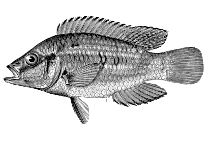
\includegraphics[width=\linewidth]{fish.png}
	\caption{An example fish.}
\end{wrapfigure}
Aliquam fringilla non diam sed varius. Suspendisse tellus felis, hendrerit non bibendum ut, adipiscing vitae diam. Lorem ipsum dolor sit amet, consectetur adipiscing elit. Nulla lobortis purus eget nisl scelerisque, commodo rhoncus lacus porta. Vestibulum vitae turpis tincidunt, varius dolor in, dictum lectus. Aenean ac ornare augue, ac facilisis purus. Sed leo lorem, molestie sit amet fermentum id, suscipit ut sem. Vestibulum orci arcu, vehicula sed tortor id, ornare dapibus lorem. Praesent aliquet iaculis lacus nec fermentum. Morbi eleifend blandit dolor, pharetra hendrerit neque ornare vel. Nulla ornare, nisl eget imperdiet ornare, libero enim interdum mi, ut lobortis quam velit bibendum nibh.

\begin{itemize}
	\item First bullet point item
	\item Second bullet point item
	\item Third bullet point item
\end{itemize}

Morbi tempor congue porta. Proin semper, leo vitae faucibus dictum, metus mauris lacinia lorem, ac congue leo felis eu turpis. Sed nec nunc pellentesque, gravida eros at, porttitor ipsum. Praesent consequat urna a lacus lobortis ultrices eget ac metus. In tempus hendrerit rhoncus. Mauris dignissim turpis id sollicitudin lacinia. Praesent libero tellus, fringilla nec ullamcorper at, ultrices id nulla. Phasellus placerat a tellus a malesuada.

\begin{enumerate}
	\item First numbered list item
	\item Second numbered list item
\end{enumerate}

%------------------------------------------------

\section*{Conclusion}

Fusce in nibh augue. Cum sociis natoque penatibus et magnis dis parturient montes, nascetur ridiculus mus. In dictum accumsan sapien, ut hendrerit nisi. Phasellus ut nulla mauris. Phasellus sagittis nec odio sed posuere. Vestibulum porttitor dolor quis suscipit bibendum. Mauris risus lectus, cursus vitae hendrerit posuere, congue ac est. Suspendisse commodo eu eros non cursus. Mauris ultrices venenatis dolor, sed aliquet odio tempor pellentesque. Duis ultricies, mauris id lobortis vulputate, tellus turpis eleifend elit, in gravida leo tortor ultricies est. Maecenas vitae ipsum at dui sodales condimentum a quis dui. Nam mi sapien, lobortis ac blandit eget, dignissim quis nunc.

Donec luctus tincidunt mauris, non ultrices ligula aliquam id. Sed varius, magna a faucibus congue, arcu tellus pellentesque nisl, vel laoreet magna eros et magna. Vivamus lobortis elit eu dignissim ultrices. Fusce erat nulla, ornare at dolor quis, rhoncus venenatis velit. Donec sed elit mi. Sed semper tellus a convallis viverra. Maecenas mi lorem, placerat sit amet sem quis, adipiscing tincidunt turpis. Cras a urna et tellus dictum eleifend. Fusce dignissim lectus risus, in bibendum tortor lacinia interdum.

\begin{table}[h] % [h] forces the table to be output where it is defined in the code (it suppresses floating)
	\caption{Example table.}
	\centering
	\begin{tabular}{l l r}
		\toprule
		\multicolumn{2}{c}{Name} \\
		\cmidrule(r){1-2}
		First Name & Last Name & Grade \\
		\midrule
		John & Doe & $7.5$ \\
		Richard & Miles & $5$ \\
		\bottomrule
	\end{tabular}
\end{table}

Fusce eleifend porttitor arcu, id accumsan elit pharetra eget. Mauris luctus velit sit amet est sodales rhoncus. Donec cursus suscipit justo, sed tristique ipsum fermentum nec. Ut tortor ex, ullamcorper varius congue in, efficitur a tellus. Vivamus ut rutrum nisi. Phasellus sit amet enim efficitur, aliquam nulla id, lacinia mauris. Quisque viverra libero ac magna maximus efficitur. Interdum et malesuada fames ac ante ipsum primis in faucibus. Vestibulum mollis eros in tellus fermentum, vitae tristique justo finibus. Sed quis vehicula nibh. Etiam nulla justo, pellentesque id sapien at, semper aliquam arcu. Integer at commodo arcu. Quisque dapibus ut lacus eget vulputate.

%----------------------------------------------------------------------------------------
%	BIBLIOGRAPHY
%----------------------------------------------------------------------------------------

\bibliographystyle{unsrt}

\begin{thebibliography}{9}
\bibitem{latexcompanion} 
Michel Goossens, Frank Mittelbach, and Alexander Samarin. 
\textit{The \LaTeX\ Companion}. 
Addison-Wesley, Reading, Massachusetts, 1993.
 
\bibitem{einstein} 
Albert Einstein. 
\textit{Zur Elektrodynamik bewegter K{\"o}rper}. (German) 
[\textit{On the electrodynamics of moving bodies}]. 
Annalen der Physik, 322(10):891–921, 1905.
 
\bibitem{knuthwebsite} 
Knuth: Computers and Typesetting,
\\\texttt{http://www-cs-faculty.stanford.edu/\~{}uno/abcde.html}
\end{thebibliography}
%----------------------------------------------------------------------------------------

\end{document}
